\documentclass[crop,border={2pt 2pt 2pt 2pt}]{standalone}
\usepackage[dvipsnames]{xcolor}
\usepackage{tikz}
\usepackage{braket}
\usepackage{bbold}
\usepackage{bm}
\usepackage{amsmath}
\usepackage{tikz-3dplot}
% \usepackage{physics}

\usetikzlibrary{backgrounds,decorations.markings, calc}
\tikzset{>=latex}
\tikzset{->-/.style={decoration={
  markings,
  mark=at position .55 with {\arrow{>}}},postaction={decorate}}}
\begin{document}
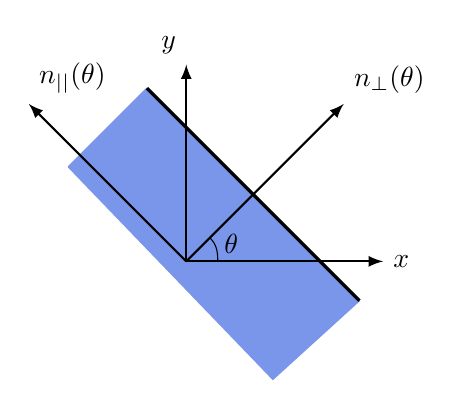
\begin{tikzpicture}[line join = round]
    \draw[fill,RoyalBlue!70!] (-0.5,2.2) -- (2.2,-0.5) -- (1.1,-1.5) -- (-1.5,1.2) -- cycle;
    \draw[very thick] (-0.5,2.2) -- (2.2,-0.5);
    \draw[thick,->] (0,0) -- (2.5,0) node[anchor=west] (x) {$x$};
    \draw[thick,->] (0,0) -- (0,2.5) node[anchor=south east] (y) {$y$};
    \draw[thick,->] (0,0) -- (2,2) node[anchor=south west] (n){$n_{\perp}(\theta)$};
    \draw[thick,->] (0,0) -- (-2,2) node[anchor=south west]{$n_{||}(\theta)$};
    \draw[black] (0.3,0.3)  [out = -45, in=90] to node[anchor=west,pos=0.3] {$\theta$} (0.4,0);
\end{tikzpicture}
\end{document}